% THE POSITIONING ERROR BUDGET.
% Each term is measured separately by scripts/measure_control_budget.py and
% the pair of bars per row is the value before and after the correction that
% was applied, so the figure shows what the corrections bought rather than
% only the state they left behind. The unmeasured term is drawn as an open
% bar with no length, because giving it one would be an invention.
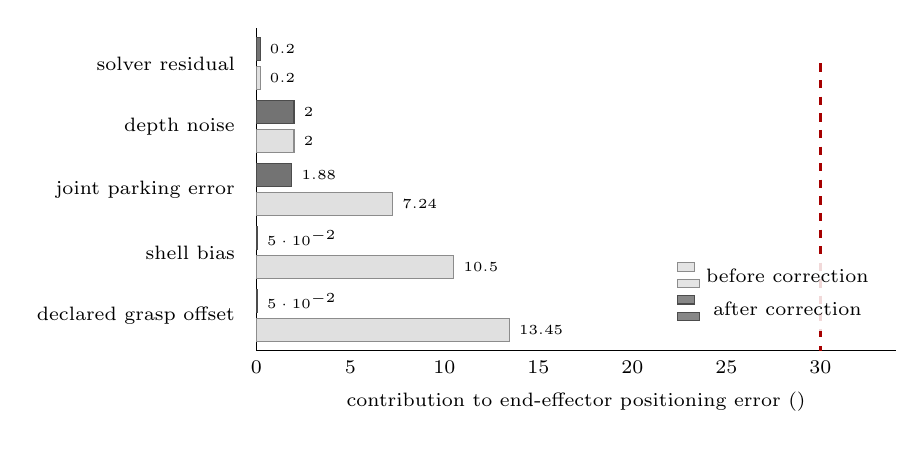
\begin{tikzpicture}
\begin{axis}[
    width=0.80\linewidth, height=64mm,
    xbar, y=8mm, bar width=3mm,
    xmin=0, xmax=34,
    xlabel={contribution to end-effector positioning error (\si{\milli\metre})},
    symbolic y coords={
      {camera mounting},
      {declared grasp offset},
      {shell bias},
      {joint parking error},
      {depth noise},
      {solver residual}},
    ytick=data,
    y tick label style={font=\scriptsize},
    x tick label style={font=\scriptsize},
    xlabel style={font=\scriptsize},
    nodes near coords, nodes near coords style={font=\tiny},
    every node near coord/.append style={anchor=west},
    enlarge y limits=0.14,
    axis lines*=left,
    tick style={draw=none},
    legend style={font=\scriptsize, at={(0.98,0.06)}, anchor=south east,
                  draw=none, fill=white, fill opacity=0.85,
                  text opacity=1, row sep=1pt},
]
\addplot[fill=black!12, draw=black!45] coordinates {
  (0.2,{solver residual})
  (2.0,{depth noise})
  (7.24,{joint parking error})
  (10.5,{shell bias})
  (13.45,{declared grasp offset})
};
\addlegendentry{before correction}
\addplot[fill=black!55, draw=black!70] coordinates {
  (0.2,{solver residual})
  (2.0,{depth noise})
  (1.88,{joint parking error})
  (0.05,{shell bias})
  (0.05,{declared grasp offset})
};
\addlegendentry{after correction}

% The unmeasured term. An open bar of no length, so it cannot be read as a
% quantity: there is no computer-aided design of the gripper module in this
% repository and the transform has never been measured.
\draw[black!55, dashed, thick] (axis cs:0,{camera mounting})
  rectangle (axis cs:9,{camera mounting});
\node[font=\tiny\itshape, anchor=west, black!55]
  at (axis cs:9.6,{camera mounting}) {not measured: the largest remaining unknown};

\draw[red!65!black, thick, dashed]
  (axis cs:30,{solver residual}) -- (axis cs:30,{camera mounting});
\node[font=\tiny, red!65!black, anchor=south east, align=right]
  at (axis cs:29.4,{camera mounting}) {\SI{30}{\milli\metre} capture gate};
\end{axis}
\end{tikzpicture}
